% Created 2020-03-12 Thu 16:26
% Intended LaTeX compiler: pdflatex
\documentclass[presentation]{beamer}
\usepackage[utf8]{inputenc}
\usepackage[T1]{fontenc}
\usepackage{graphicx}
\usepackage{grffile}
\usepackage{longtable}
\usepackage{wrapfig}
\usepackage{rotating}
\usepackage[normalem]{ulem}
\usepackage{amsmath}
\usepackage{textcomp}
\usepackage{amssymb}
\usepackage{capt-of}
\usepackage{hyperref}
\usepackage{awesomebox}
\usepackage{booktabs}
\usepackage{placeins}
\usepackage{siunitx}
\usepackage{minted}
\usetheme[progressbar=frametitle]{metropolis}
\usepackage{tikz}
\usetikzlibrary{backgrounds,matrix,fit,calc}
\usepackage{pgfplots}
\pgfplotsset{compat=1.16}
\usepackage{nicematrix}
\usepackage{spot}
\usepackage[beamer,customcolors]{hf-tikz}
\newcommand{\gv}[1]{\ensuremath{\mbox{\boldmath$ #1 $}}}
\newcommand{\bv}[1]{\ensuremath{\mathbf{#1}}}
\newcommand{\norm}[1]{\left\lVert#1\right\rVert}
\newcommand{\order}[1]{\mathcal O \left( #1 \right)} % order of magnitude
\newcommand*{\Scale}[2][4]{\scalebox{#1}{$#2$}}%
\definecolor{scarlet}{rgb}{1.0, 0.13, 0.0}
\definecolor{shamrockgreen}{rgb}{0.0, 0.62, 0.38}
\definecolor{royalblue}{rgb}{0.25, 0.41, 0.88}
\definecolor{metropolisorange}{RGB}{235,129,27}
\definecolor{deeppink}{RGB}{205,16,118}
\definecolor{burple}{RGB}{104,50,227}
\setmonofont{Iosevka Semibold}
\usetheme{default}
\author{\emph{Tejaswin Parthasarathy}, Mattia Gazzola}
\date{\today}
\title{Covariance Matrix Adaptation in Python}
\subtitle{ME498: Comp. modeling \& optimization}
\hypersetup{
 pdfauthor={\emph{Tejaswin Parthasarathy}, Mattia Gazzola},
 pdftitle={Covariance Matrix Adaptation in Python},
 pdfkeywords={},
 pdfsubject={},
 pdfcreator={Emacs 27.0.50 (Org mode 9.2)},
 pdflang={English}}
\begin{document}

\maketitle
\pgfplotsset{
colormap={whitered}{color(0cm)=(white); rgb255(1cm)=(235,129,27)}
}
\section{Some ``realistic'' examples}
\label{sec:org55be177}
\begin{frame}[label={sec:orge55e1ac}]{Brachistochrone problem}
\begin{columns}
\begin{column}{0.5\columnwidth}
\begin{figure}[htbp]
\centering
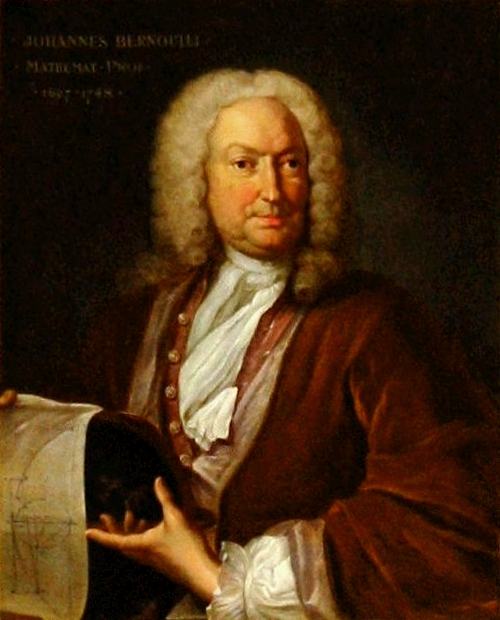
\includegraphics[width=.9\linewidth]{images/Johann_Bernoulli2.jpg}
\caption{Johannes Bernoulli}
\end{figure}
\end{column}
\begin{column}{0.5\columnwidth}
\begin{center}
	\begin{tikzpicture}[baseline,scale=1.2]
	\draw [-latex] (-0.5, 0) -- (4, 0) node [right] {$x$};
	\draw [-latex] (0, 0.5) -- (0, -2) node [below] {$y$};

	%\node [circle,fill=black,inner sep=0pt,minimum size=3pt,label=below:{$\frac{3}{2}$}] (a) at (2/3,0) {};
	\node [anchor = south east] (a) {$A$};

	%\node at (3, -1) [circ] {};
	\node at (3, -1) [right] (b) {$B$};
	\draw [thick, black] (0, 0) parabola bend (2, -1.5) (3, -1);
	\draw [thin, gray, dashed] (0, 0) -- (3, -1);
	\draw [black, fill=black] circle [radius=0.05];
	\draw [black, fill=black] (3,-1) circle [radius=0.05];
	\draw [black, fill=metropolisorange] (0.86, -1) circle [radius=0.1];
	\node at (2, -1.5) [below] {$y = f(x)$};
	\draw [->] (3.8, -0.5) -- (3.8, -1.8) node [below] {$\gv{g}$};
	\end{tikzpicture}
\end{center}
\(\beta \rho \acute{\alpha} \chi \iota \sigma \tau o \varsigma\)
(\emph{brachistos} or shortest) \(\chi
	\rho \acute{o} \nu o \varsigma\) (\emph{chronos} or time)
\end{column}
\end{columns}
\end{frame}
\begin{frame}[label={sec:org3acb4ea}]{Brachistochrone problem}
\begin{columns}
\begin{column}{0.35\columnwidth}
\begin{center}
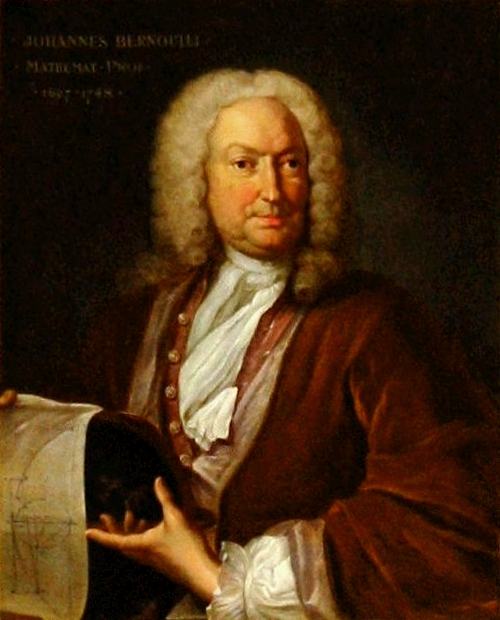
\includegraphics[width=.9\linewidth]{images/Johann_Bernoulli2.jpg}
\end{center}
\end{column}
\begin{column}{0.7\columnwidth}
\begin{quotation} %% :B\_quotation:BMCOL:
{\small ``I, Johann Bernoulli, address the most brilliant mathematicians in the
world..... Following the example set by Pascal, Fermat, etc., I hope to
gain the gratitude of the whole scientific community by placing before the
finest mathematicians of our time a problem which will test their methods and
the strength of their intellect..."}

{\small ``...Given two points A and B in a vertical plane, what is the curve traced out by a
point acted on only by gravity, which starts at A and reaches B in the shortest time."}
\end{quotation}
\end{column}
\end{columns}
\end{frame}

\begin{frame}[label={sec:org1291853}]{Brachistochrone problem : more formally}
\begin{center}
	\begin{tikzpicture}[baseline, scale=0.8]
	\draw [-latex] (-0.5, 0) -- (4, 0) node [right] {$x$};
	\draw [-latex] (0, 0.5) -- (0, -2) node [below] {$y$};

	%\node [circle,fill=black,inner sep=0pt,minimum size=3pt,label=below:{$\frac{3}{2}$}] (a) at (2/3,0) {};
	\node [anchor = south east] (a) {$A$};

	%\node at (3, -1) [circ] {};
	\node at (3, -1) [right] (b) {$B$};
	\draw [thick, black] (0, 0) parabola bend (2, -1.5) (3, -1);
	\draw [thin, gray, dashed] (0, 0) -- (3, -1);
	\draw [black, fill=black] circle [radius=0.05];
	\draw [black, fill=black] (3,-1) circle [radius=0.05];
	\draw [black, fill=metropolisorange] (0.86, -1) circle [radius=0.1];
	\node at (2, -1.5) [below] {$y = f(x)$};
	\draw [->] (3.8, -0.5) -- (3.8, -1.8) node [below] {$\gv{g}$};
	\end{tikzpicture}
\end{center}
\begin{definition}[Brachistochrone problem]
For \(x : [x_A, x_B]\), let
\(\mathbf{x} \mapsto \begin{pmatrix} x \\ y(x) \end{pmatrix},
	 y : [0, x] \to \mathbb{R}\) with BoCos.

Find \(y^*  = \mathop{\mathrm{arg\,min}_y} L[y] \mathrel{\mathop:}= t_B(y, y',y'')\) where
\(t : \mathbb{R}^3 \to \mathbb{R}^+\) is trajectory time.
\begin{block}{In the context of optimization \(\left( \mathcal{C}^2, \mathbb{R}, f, \leq \right)\)}
By solving \(\ddot{x} = \frac{g_x + y' \left[ g_y - y'' \dot{x}^2 \right]}{1 + y'^2}\)
with \(x(A) = x_A, \dot{x}(A) = 0\) to obtain \(x = f(t, y, y', y''')\).
Then \(t \mathrel{\mathop:}= f^{-1}(x, y, y', y''')\)
\end{block}
\end{definition}
\end{frame}
\begin{frame}[label={sec:orgdcd5c8d}]{Requirements}
\begin{alertblock}{Simulation}
\begin{itemize}
\item \alert{Numerical solution} of non-linear Ordinary Differential Equation (ODE)
\end{itemize}
\end{alertblock}
\begin{alertblock}{Optimization problem}
\begin{itemize}
\item \alert{Representation} of \(\mathcal{C}^2\)
\item Definition of \alert{fitness function}
\item Black-box \alert{optimizer} (we pick CMAes in this case)
\item \alert{Constraints} on domain and range
\begin{itemize}
\item not all \(\mathcal{C}^2\) are feasible (boundary conditions!)
\end{itemize}
\end{itemize}
\end{alertblock}
\end{frame}
\begin{frame}[label={sec:org81e85da},fragile]{ODE solver}
 \begin{definition}[Ordinary Differential Equation]
\[ \frac{dy}{dt} = f(t, y, y', \dots, y^{k})\]
accompanied by \(k\) initial conditions \(\Rightarrow\) solved by \(y(t)\).
\begin{itemize}
\item Few non-linear problems can be solved analytically \(\Rightarrow\) \alert{numerical methods}
\item \emph{Timesteppers}---Euler, Runge-Kutta etc.
\end{itemize}
\end{definition}
\begin{example}[Scipy's ODE solver]
\begin{itemize}
\item \texttt{scipy.integrate.solve\_ivp} \alert{DEMO}
\item many options \texttt{RK23, RK45, BDF,...}
\item can specify error tolerances \texttt{rtol}, \texttt{atol}
\end{itemize}
\end{example}
\end{frame}
\begin{frame}[label={sec:org4ae8c51}]{Representation}
\begin{block}{Function space \(\mathcal{C}^2 \to \mathbb{R}\)?}
\begin{itemize}
\item Our optimizer works ONLY with real numbers
\end{itemize}
\end{block}
\begin{block}{Linear combination of basis functions}
\begin{itemize}
\item \(\forall x \in D\), \(f(x) = \sum_{i=1}^{N} c_i \phi_i(x)\)
\item look for \emph{good} values of \(c_i\)
\end{itemize}
\end{block}
\begin{columns}
\begin{column}{0.32\columnwidth}
\begin{center}
	\begin{tikzpicture}[scale=0.48]
		\begin{axis}[
					title={Polynomial bases},
					xmin=0,
					xmax=1,
					ymin=-1.05,
					ymax=1.05,
					samples=50,
					xlabel={$s$},
					ylabel={$\phi(s)$},
					ylabel shift = -10 pt]
			 \addplot[royalblue,  ultra thick, domain=0:1] {x};
			 \addplot[scarlet, ultra thick, domain=0:1] {x^2};
			 \addplot[black,  ultra thick, domain=0:1] {x^3};
			 \addplot[metropolisorange,  ultra thick, domain=0:1] {x^4};
			 \addplot[shamrockgreen,  ultra thick, domain=0:1] {x^5};
			 \addplot[deeppink,  ultra thick, domain=0:1] {x^6};
			 \addplot[burple,  ultra thick, domain=0:1] {1};
			 \draw[ultra thin] (axis cs:\pgfkeysvalueof{/pgfplots/xmin},0) -- (axis cs:\pgfkeysvalueof{/pgfplots/xmax},0);
		\end{axis}
	\end{tikzpicture}
\end{center}
\end{column}
\begin{column}{0.32\columnwidth}
\begin{center}
	\begin{tikzpicture}[scale=0.48]
		\begin{axis}[
					title={Fourier bases},
					xmin=0,
					xmax=1,
					ymin=-1.05,
					ymax=1.05,
					samples=50,
					xlabel={$s$}]
			\addplot[royalblue, ultra thick, domain=0:1] {sin(deg(pi * x))};
			\addplot[scarlet, ultra thick, domain=0:1] {cos(deg(pi * x))};
			\addplot[black,  ultra thick, domain=0:1] {sin(deg(2.0 * pi * x))};
			\addplot[metropolisorange,  ultra thick, domain=0:1] {cos(deg(2.0 * pi * x)))};
			\addplot[shamrockgreen,  ultra thick, domain=0:1] {sin(deg(3.0 * pi * x))};
			\addplot[deeppink,  ultra thick, domain=0:1] {cos(deg(3.0 * pi * x)))};
			\addplot[burple,  ultra thick, domain=0:1] {1};

			\draw[ultra thin] (axis cs:\pgfkeysvalueof{/pgfplots/xmin},0) -- (axis cs:\pgfkeysvalueof{/pgfplots/xmax},0);
		\end{axis}
	\end{tikzpicture}
\end{center}
\end{column}
\begin{column}{0.32\columnwidth}
\begin{center}
	\begin{tikzpicture}[scale=0.48]
		\begin{axis}[
					title={B-splines},
					xmin=0,
					xmax=1,
					ymin=-1.05,
					ymax=1.05,
					samples=50,
					xlabel={$s$}]
				% Taken from https://pages.mtu.edu/~shene/COURSES/cs3621/NOTES/spline/B-spline/bspline-ex-1.html
				% N02
				\addplot[royalblue, ultra thick, domain=0:0.3] {(1 - (10/3)*x)^2 };

				% N12
				\addplot[scarlet, ultra thick, domain=0:0.3] {(20/3)*(x - (8/3)*x^2)  };
				\addplot[scarlet, ultra thick, domain=0.3:0.5] {2.5*(1.0 - 2*x)^2};

				% N22
				\addplot[black, ultra thick, domain=0:0.3] {(20/3)*x^2  };
				\addplot[black, ultra thick, domain=0.3:0.5] {-3.75 + 25*x - 35*x^2};

				% N32
				\addplot[metropolisorange,  ultra thick, domain=0.3:0.5] {(5*x - 1.5)^2};
				\addplot[metropolisorange,  ultra thick, domain=0.5:0.6] {(6 - 10 * x)^2};

				% N42
				\addplot[shamrockgreen,  ultra thick, domain=0.5:0.6] {20 * (-2 + 7*x - 6*x^2) };
				\addplot[shamrockgreen,  ultra thick, domain=0.6:1] {5*(1 - x)^2};

				% N52
				\addplot[deeppink,  ultra thick, domain=0.5:0.6] {20*x^2 - 20*x + 5 };
				\addplot[deeppink,  ultra thick, domain=0.6:1] {-11.25*x^2 + 17.5*x - 6.25};

				% N52
				\addplot[burple,  ultra thick, domain=0.6:1] {6.25*x^2 - 7.5*x + 2.25};

				\draw[ultra thin] (axis cs:\pgfkeysvalueof{/pgfplots/xmin},0) -- (axis cs:\pgfkeysvalueof{/pgfplots/xmax},0);
		\end{axis}
	\end{tikzpicture}
\end{center}
\end{column}
\end{columns}
\end{frame}
\begin{frame}[label={sec:org3734b08}]{Representation}
\begin{itemize}
\item See\href{http://jsxgraph.uni-bayreuth.de/wiki/index.php/B-splines}{ this link} (B-splines) and \href{https://bl.ocks.org/jinroh/7524988}{this} link + \href{https://www.youtube.com/watch?v=spUNpyF58BY}{this video} for a visual understanding of the different bases functions.
\end{itemize}
\end{frame}
\begin{frame}[label={sec:org755cfcf}]{Fitness function}
\begin{block}{What's the fitness?}
\begin{itemize}
\item <2-> Measure time at \(x(t) = x_B\)
\end{itemize}
\end{block}
\begin{columns}
\begin{column}{0.3\columnwidth}
\begin{center}
	\begin{tikzpicture}[scale=0.48]
	\begin{axis}[
		grid=major, % Display a grid
		grid style={dashed,gray!30}, % Set the style
		xlabel=$x$, % Set the labels
		% ylabel=$y$,
		ymin=-1.05,
		ymax=0.05
		]
		\node at (axis cs:0,0) [left] (a) {$A$};
		\node at (axis cs:1, -1) [right] (b) {$B$};
		% \draw [black, fill=black] (axis cs:0, 0) circle [radius=0.01];
		% \draw [black, fill=black] (axis cs:1,-1) circle [radius=0.01];
		\addplot[line width=2pt, metropolisorange, mark=none]
		% add a plot from table; you select the columns by using the actual name in
		% the .csv file (on top)
		table[col sep=comma] {data_from_optex/first_spline_profile.csv};
		\addplot[only marks, mark=*]
		table[col sep=comma] {data_from_optex/first_spline_time.csv};
	\end{axis}
	\end{tikzpicture}
\end{center}
\begin{itemize}
\item <2->\(f = \SI{0.638}{\s}\)
\end{itemize}
\end{column}
\begin{column}{0.3\columnwidth}
\begin{center}
	\begin{tikzpicture}[scale=0.48]
	\begin{axis}[
		grid=major, % Display a grid
		grid style={dashed,gray!30}, % Set the style
		xlabel=$x$, % Set the labels
		ymin=-1.05,
		ymax=0.05
		]
		\node at (axis cs:0,0) [left] (a) {$A$};
		\node at (axis cs:1, -1) [right] (b) {$B$};
		% \draw [black, fill=black] (axis cs:0, 0) circle [radius=0.01];
		% \draw [black, fill=black] (axis cs:1,-1) circle [radius=0.01];
		\addplot[line width=2pt, royalblue, mark=none]
		% add a plot from table; you select the columns by using the actual name in
		% the .csv file (on top)
		table[col sep=comma] {data_from_optex/second_spline_profile.csv};
		\addplot[only marks, mark=*]
		table[col sep=comma] {data_from_optex/second_spline_time.csv};
	\end{axis}
	\end{tikzpicture}
\end{center}

\begin{itemize}
\item <2->\(f = \SI{0.713}{\s}\)
\end{itemize}
\end{column}
\begin{column}{0.3\columnwidth}
\begin{center}
	\begin{tikzpicture}[scale=0.48]
	\begin{axis}[
		grid=major, % Display a grid
		grid style={dashed,gray!30}, % Set the style
		xlabel=$x$, % Set the labels
		ymin=-1.05,
		ymax=0.05
		]
		\node at (axis cs:0,0) [left] (a) {$A$};
		\node at (axis cs:1, -1) [right] (b) {$B$};
		% \draw [black, fill=black] (axis cs:0, 0) circle [radius=0.01];
		% \draw [black, fill=black] (axis cs:1,-1) circle [radius=0.01];
		\addplot[line width=2pt, scarlet, mark=none]
		% add a plot from table; you select the columns by using the actual name in
		% the .csv file (on top)
		table[col sep=comma] {data_from_optex/optimal_spline_profile.csv};
		\addplot[only marks, mark=*]
		table[col sep=comma] {data_from_optex/optimal_spline_time.csv};
	\end{axis}
	\end{tikzpicture}
\end{center}
\begin{itemize}
\item <2->\(f = \SI{0.585}{\s}\)
\end{itemize}
\end{column}
\end{columns}
\end{frame}
\begin{frame}[label={sec:org66e9ba2}]{Constraints and penalties}
\begin{block}{Is unconstrained optimization a good idea?}
\begin{itemize}
\item <2-> \alert{NO}! We penalize \emph{bad} solutions.
\end{itemize}
\end{block}
\begin{columns}
\begin{column}{0.5\columnwidth}
\begin{center}
	\begin{tikzpicture}[scale=0.65]
	\begin{axis}[
		grid=major, % Display a grid
		grid style={dashed,gray!30}, % Set the style
		xlabel=$x$, % Set the labels
		ylabel=$y$,
		ymin=-2.2,
		ymax=0.2
		]
		\node at (axis cs:0,0) [left] (a) {$A$};
		\node at (axis cs:1, -1) [right] (b) {$B$};
		% Different radii because its uneven
		\draw [black, fill=black] (axis cs:0, 0) circle [x radius=0.02, y radius=0.04];
		\draw [black, fill=black] (axis cs:1,-1) circle [x radius=0.02, y radius=0.04];
		\addplot[line width=2pt, scarlet, mark=none]
		% add a plot from table; you select the columns by using the actual name in
		% the .csv file (on top)
		table[col sep=comma] {data_from_optex/positive_slope_spline_profile.csv};
	\end{axis}
	\end{tikzpicture}
\end{center}
\begin{itemize}
\item <2-> Positive slope : simulation \emph{fails}
\end{itemize}
\end{column}
\begin{column}{0.5\columnwidth}
\begin{center}
	\begin{tikzpicture}[scale=0.65]
	\begin{axis}[
		grid=major, % Display a grid
		grid style={dashed,gray!30}, % Set the style
		xlabel=$x$, % Set the labels
		ylabel=$y$,
		ymin=-2.2,
		ymax=0.2
		]
		\node at (axis cs:0,0) [left] (a) {$A$};
		\node at (axis cs:1, -1) [right] (b) {$B$};
		\draw [black, fill=black] (axis cs:0, 0) circle [x radius=0.02, y radius=0.04];
		\draw [black, fill=black] (axis cs:1,-1) circle [x radius=0.02, y radius=0.04];
		\addplot[line width=2pt, royalblue, mark=none]
		% add a plot from table; you select the columns by using the actual name in
		% the .csv file (on top)
		table[col sep=comma] {data_from_optex/third_spline_profile.csv};
		\only<2->{\draw[fill=metropolisorange, fill opacity=0.2] (axis cs:0, 0) rectangle (axis cs:1,-1.3)};
	\end{axis}
	\end{tikzpicture}
\end{center}
\begin{itemize}
\item <2-> Need realistic bounds on coefficients!
\end{itemize}
\end{column}
\end{columns}
\end{frame}
\begin{frame}[label={sec:org848caf1}]{Results}
\href{file:///Users/tp5/code/optex/brachistochrone.mp4}{Brachistochrone optimization}
\end{frame}
\begin{frame}[label={sec:org3c95edd}]{Additional discussion}
Think about how these choices affect the optimization campaign?
\begin{block}{Population size / number of generations}
\end{block}
\begin{block}{Number of spline parameters (aka the dimensionality of the problem)?}
\end{block}
\begin{block}{Penalization coefficients?}
\end{block}
\begin{block}{Optimize ``part'' of the problem?}
\end{block}
\begin{block}{Error tolerance of ODE solver?}
\end{block}
\end{frame}
\begin{frame}[label={sec:orgfe9cd15}]{Aliters}
\begin{columns}
\begin{column}{0.4\columnwidth}
\begin{block}{Johann's solution}
\begin{itemize}
\item Geometrical
\item Energy conservation
\item Shady (af).
\end{itemize}
\end{block}
\end{column}
\begin{column}{0.6\columnwidth}
\begin{block}{Jakob Bernoulli's solution}
\begin{itemize}
\item Snell's law!
\item Led eventually to calculus of variations
\end{itemize}
\end{block}
\end{column}
\end{columns}
\begin{block}{Isaac Newton's solution}
\begin{itemize}
\item Minimal resistance problem
\end{itemize}
\end{block}
\begin{block}{Calculus of variations / optimal control theory}
\begin{itemize}
\item \(y^*  = \mathop{\mathrm{arg\,min}_y} L[y] \mathrel{\mathop:}=
       \displaystyle\int_{x_A}^{x_B} \dfrac{\sqrt{1 + (y'(x))^2}}{\sqrt{y(x)}}
      dx\)
\end{itemize}
\end{block}
\begin{block}{The optimal solution is a cycloid!}
\end{block}
\end{frame}
\begin{frame}[label={sec:org489473d}]{More history\footnote{\href{https://en.wikipedia.org/wiki/Brachistochrone\_curve}{Brachistochrone curve wiki}}}
\footnotesize
\begin{itemize}
\item Johann Bernoulli allowed six months for other solutions (apart from his and
Jakob's)
\item At the request of Leibniz, the time was publicly extended for a year and a
half.
\item At 4 p.m. on 29 January 1697 when he arrived home from the Royal Mint,
Isaac Newton found the challenge in a letter from Johann Bernoulli.
\item Newton stayed up all night to solve it and mailed the solution anonymously
by the next post
\item Upon reading the solution, Bernoulli recognized its author, exclaiming that
he ``recognizes a lion from his claw mark''
\item Johann had taken two weeks to solve the same problem
\item Newton also wrote, ``I do not love to be dunned [pestered] and teased by
foreigners about mathematical things\ldots{}''
\item In the end, five mathematicians responded with solutions: Newton,
Bernoulli(s), Leibniz, Tschirnhaus and l'Hôpital.
\end{itemize}
\end{frame}
\begin{frame}[label={sec:org32b8140}]{Dido's isoperimetric problem\footnote{\href{https://mathematicalgarden.wordpress.com/2008/12/21/the-problem-of-dido/}{Mathematical Garden}}}
\begin{block}{Constraints in the problem definition}
What is the closed curve which has the maximum area for a given perimeter?

\begin{center}
	\begin{tikzpicture}[scale=0.65]
	\begin{axis}[axis equal,
		grid=major, % Display a grid
		grid style={dashed,gray!30}, % Set the style
		xlabel=$x$, % Set the labels
		ylabel=$f(x)$,
		xmin=0,
		xmax=1,
		ymin=0,
		ymax=0.6,
		samples=100]
		\addplot[royalblue,  line width=3pt, domain=0:1] {(0.25-(x-0.5)^2)^0.5};

		\addplot[metropolisorange,  line width=3pt, domain=0:0.5] {2.8*(x-1.5*x^2)};
		\addplot[metropolisorange,  line width=3pt, domain=0.5:1] {1.4*(1-x)^2};

		\addplot[black,  line width=3pt, domain=0.0:0.5] {1.4*x^2};
		\addplot[black,  line width=3pt, domain=0.5:1.0] {2.8*(-0.5-1.5*x^2+2*x)};

	\end{axis}
	\end{tikzpicture}
\end{center}
\end{block}
\end{frame}
\begin{frame}[label={sec:org9416b59}]{Results}
\begin{itemize}
\item Constraint satsifaction by pre-processing and not by repair
\item \href{file:///Users/tp5/code/optex/isoperimetric.mp4}{Isoperimetric curve optimization}
\end{itemize}
\end{frame}
\end{document}
